% !TEX root =  ../main_manuscript.tex 
\subsection{Statistical Methods}
Our aim was to develop a model for predicting the time of GS7. The available data for each patient were, age at the start of AS, all observed PSA measurements, and the history of biopsies. The PSA measurements of a patient were measured longitudinally and were likely correlated. They could also be higher when measured closer to the time of GS7. An additional complication was that such higher values were often missing once a patient obtained GS7. The vice versa, that is, GS7 could be indicated by rise in PSA was also plausible. Such complex correlations between a longitudinal PSA outcome and a time of GS7 outcome are commonly modeled via a joint model for time-to-event and longitudinal data \citep{rizopoulos2012joint,tomer2019,coley2017prediction}.

\begin{figure}[!htb]
\centerline{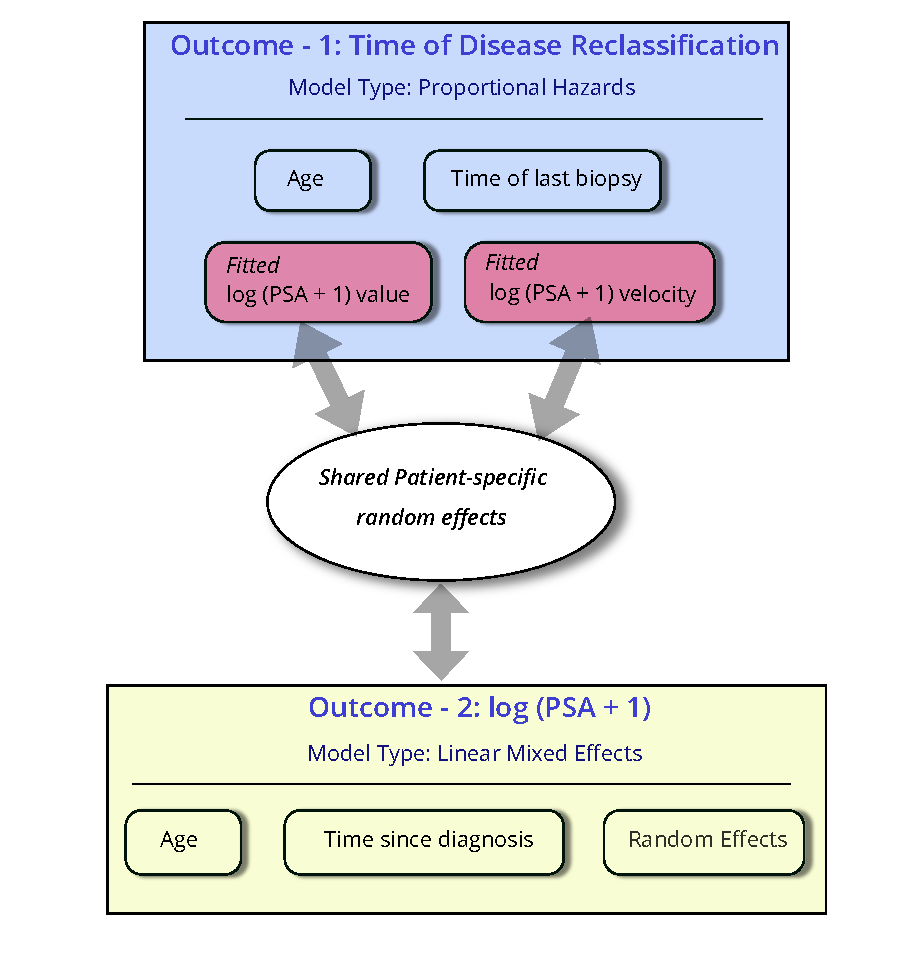
\includegraphics[width=\columnwidth]{images/jm_blockdiag.pdf}}
\caption{\textbf{Diagram of the joint model}: Patient-specific random effects (ellipse in center) are shared between sub-models for all outcomes pertaining to prostate cancer progression, to model the correlation between them. In the linear mixed effects sub-model for $\log_2\{\mbox{PSA + 1}\}$ transformed PSA outcome (bottom rectangle), random effects are used as covariates. In the relative-risk sub-model (similar to Cox model) for time of Gleason~$\geq$~7 (GS7), random effects are utilized indirectly, by including fitted $\log_2\{\mbox{PSA + 1}\}$ value and velocities as covariates. Age of patient at baseline is included in both sub-models. Parameters of both sub-models are estimated jointly.}
\label{fig:jm_blockdiag}
\end{figure}

Our joint model exploited patient-specific random effects \citep{laird1982random} to act as a common source of correlation between the sub-models for the PSA and time of GS7 outcomes (see Figure~\ref{fig:jm_blockdiag}). Random effects manifested the underlying state of PCa, and were included in both the linear mixed effects sub-model for $\log_2\{\mbox{PSA + 1}\}$ transformed measurements, and the relative risk sub-model (similar to cox model) for time of GS7. In the PSA sub-model, random effects non-linearly modeled the evolution of PSA over time. Simultaneously, in the relative risk model they were included indirectly by using fitted $\log_2\{\mbox{PSA + 1}\}$ value and velocity as time dependent covariates. This established the correlation between PSA and time of GS7. Unlike observed $\log_2\{\mbox{PSA + 1}\}$ values, the fitted values were free of measurement errors. The $\log_2\{\mbox{PSA + 1}\}$ velocity was mathematically derived from fitted $\log_2\{\mbox{PSA + 1}\}$ values. The $\log_2\{\mbox{PSA + 1}\}$ velocity was also allowed to change non-linearly over follow-up.

The parameters of the two sub-models were estimated jointly using the R \textbf{JMbayes} \citep{rizopoulosJMbayes}. This package utilizes the Bayesian methodology to estimate model parameters. The parameters and 95\% credible intervals are presented in Table.. of Appendix.

\subsection{Assessment of Predictions}
We assessed the goodness of fit of our model using both in-sample and out-of-sample predictions of GS7. For out-of-sample predictions we utilized the five largest AS cohorts that constitute the GAP3 database \citep{gap3_2018}. We measured the accuracy of these predictions via the root mean squared prediction error or RMSPE \cite{rizopoulos2017dynamic} and the area under the receiver operating characteristic curve or AUC \cite{rizopoulos2017dynamic}. Both of these measures take a value between zero and one. The RMSPE is a measure of calibration representing the difference between the true GS7 status of a patient, and the predicted risk of GS7. Ideally the RMSPE should be zero. The AUC indicates if the model is able to discriminate between patients who obtain GS7 and those do not obtain it. Ideally it should be equal to one. In practice it should not be less than 0.5 (AUC of random discrimination). Since PRIAS is a longitudinal study, we compute these measures in a time dependent manner, at a gap of every one year until xx years of follow-up (95\% quantile of observed GS7 times).

\subsection{Estimate Risk of GS7 and Consequences of Biopsies}
Consider a new patient P shown in Figure .... Using the joint model fitted to the PRIAS dataset, we first obtained his profile of the cumulative risk of GS7 over the follow-up period. We then suggest a biopsy at a follow-up visit if the cumulative risk at that visit is above a certain threshold (e.g., 10\% risk). The cumulative risk is updated at each new visit, by accounting for latest PSA measurements and decisions of biopsies. One can then repeatedly apply the threshold based decision rule for biopsies at each new visit. 

The choice of a threshold is not easy. To this end, we exploit the entire cumulative risk profile of a patient to estimate the consequences of following a particular threshold based schedule (Figure ...). The consequences we use in this paper are the expected delay in detection of GS7, the corresponding number of biopsies required, at the estimated visit times at which they are scheduled. These estimates are patient specific and also updated with new data at each visit. Since we calculate the consequences for various fixed biopsy schedules as well, patients can make a more informed decision of biopsy. Lastly, we implemented this approach in a web-based application for use in medical centers.